% Q3V4: Rectangular Core, Opposing Dots, Tight Coupling — Physical winding diagram
% Coils wound in OPPOSITE DIRECTIONS on rectangular core
% Coil 1 on top (CW from viewer), Coil 2 on bottom (CCW from viewer)
% Does NOT show dot placements — that is Part (a) answer (P-STACK-31)
\documentclass[border=10pt]{standalone}
\usepackage{tikz}
\usepackage{amsmath}
\renewcommand{\familydefault}{\sfdefault}

\begin{document}
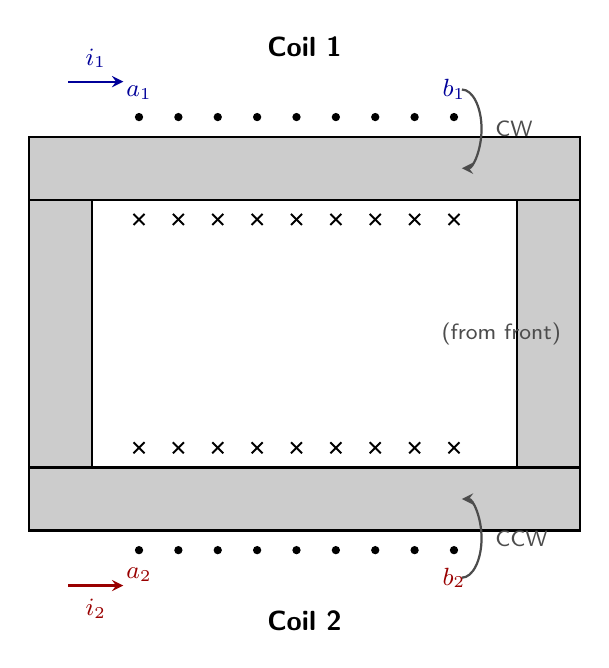
\begin{tikzpicture}[
    every node/.style={font=\sffamily},
    >=stealth,
]

% === Rectangular core (no gaps) ===
\def\coreW{7}
\def\coreH{5}
\def\limbW{0.8}

% Top yoke
\fill[gray!40, draw=black, line width=0.8pt]
    (0,{\coreH-\limbW}) rectangle (\coreW,\coreH);
% Bottom yoke
\fill[gray!40, draw=black, line width=0.8pt]
    (0,0) rectangle (\coreW,\limbW);
% Left limb
\fill[gray!40, draw=black, line width=0.8pt]
    (0,\limbW) rectangle (\limbW,{\coreH-\limbW});
% Right limb
\fill[gray!40, draw=black, line width=0.8pt]
    ({\coreW-\limbW},\limbW) rectangle (\coreW,{\coreH-\limbW});

% === Coil 1 (top section) — clockwise from viewer ===
% CW from front view → dots on top (out of page), crosses on bottom (into page)
\foreach \xcoil in {1.4, 1.9, 2.4, 2.9, 3.4, 3.9, 4.4, 4.9, 5.4} {
    % Top side: dot (out of page)
    \fill (\xcoil,{\coreH+0.25}) circle (1.5pt);
    % Bottom side: cross (into page)
    \draw[line width=0.7pt] ({\xcoil-0.07},{\coreH-\limbW-0.32}) -- ({\xcoil+0.07},{\coreH-\limbW-0.18});
    \draw[line width=0.7pt] ({\xcoil-0.07},{\coreH-\limbW-0.18}) -- ({\xcoil+0.07},{\coreH-\limbW-0.32});
}

% Coil 1 labels (spaced: terminal labels at dot level, current arrow above)
\node[above, font=\sffamily\bfseries] at ({0.5*\coreW},{\coreH+0.9}) {Coil 1};
\node[above, font=\sffamily\small, text=blue!60!black] at (1.4,{\coreH+0.35}) {$a_1$};
\node[above, font=\sffamily\small, text=blue!60!black] at (5.4,{\coreH+0.35}) {$b_1$};

% Current arrow for Coil 1 (above terminal labels)
\draw[->, thick, blue!60!black] (0.5,{\coreH+0.7}) -- (1.2,{\coreH+0.7});
\node[above, font=\sffamily\small, text=blue!60!black] at (0.85,{\coreH+0.75}) {$i_1$};

% === Coil 2 (bottom section) — OPPOSITE direction (CCW from viewer) ===
% CCW from front → crosses on top (into page), dots on bottom (out of page)
% NOTE: reversed from Coil 1!
\foreach \xcoil in {1.4, 1.9, 2.4, 2.9, 3.4, 3.9, 4.4, 4.9, 5.4} {
    % Top side: CROSS (reversed from Coil 1)
    \draw[line width=0.7pt] ({\xcoil-0.07},{\limbW+0.18}) -- ({\xcoil+0.07},{\limbW+0.32});
    \draw[line width=0.7pt] ({\xcoil-0.07},{\limbW+0.32}) -- ({\xcoil+0.07},{\limbW+0.18});
    % Bottom side: DOT (reversed from Coil 1)
    \fill (\xcoil,{-0.25}) circle (1.5pt);
}

% Coil 2 labels (spaced: terminal labels at dot level, current arrow below)
\node[below, font=\sffamily\bfseries] at ({0.5*\coreW},{-0.9}) {Coil 2};
\node[below, font=\sffamily\small, text=red!60!black] at (1.4,{-0.35}) {$a_2$};
\node[below, font=\sffamily\small, text=red!60!black] at (5.4,{-0.35}) {$b_2$};

% Current arrow for Coil 2 (below terminal labels)
\draw[->, thick, red!60!black] (0.5,{-0.7}) -- (1.2,{-0.7});
\node[below, font=\sffamily\small, text=red!60!black] at (0.85,{-0.75}) {$i_2$};

% === Winding sense annotations ===
% Coil 1: CW from front
\draw[->, thick, gray!60!black] ({0.5*\coreW+2.0},{\coreH+0.6}) arc[start angle=90, end angle=-90, x radius=0.25, y radius=0.5];
\node[right, font=\sffamily\footnotesize, gray!60!black] at ({0.5*\coreW+2.3},{\coreH+0.1}) {CW};

% Coil 2: CCW from front
\draw[->, thick, gray!60!black] ({0.5*\coreW+2.0},{-0.6}) arc[start angle=-90, end angle=90, x radius=0.25, y radius=0.5];
\node[right, font=\sffamily\footnotesize, gray!60!black] at ({0.5*\coreW+2.3},{-0.1}) {CCW};

\node[font=\sffamily\footnotesize, gray!60!black] at ({0.5*\coreW+2.5},{0.5*\coreH}) {(from front)};

\end{tikzpicture}
\end{document}
